
\mysection{Necromancy}{arcana-necromancy}

To reach through the veil between life and death is to plunge your hands into the black rivers surrounding the Isle of the Dead.  Necromancy is abhorrent to Hallowed creatures; there are those who insist that Necromancy defies \TheAuthority, while others insist that it would not be possible if it were not permitted.  


Necromancy requires the \mylink{Crux of Mojo}{mortal-crux-mojo}, and is divided into three loose groups:  Black Magic, Carnomancy, and Corpse Witching.  Each Necromantic spell has a "Target" associated with it - you must roll this number or greater using your Mojo.  You can try as many times as you like, but if you roll a 1 or a 2, your Mojo moves \DCDOWN.  Rolling your Mojo in this way is a Maneuver Action.


\mysubsection{Black Magic}{arcana-necromancy-black-magic}

\NECRO[
  Name=Born of the Grave,
  Link=necromancy-born-of-the-grave,
  Paradigm=Death,
  Save=N,
  Duration=Session,
  Target=4
]

Requires a snort of \mylink{Corpse Salt}{necromancy-corpse-salt}.  In addition to the Salt's narcotic abilities (see the Core Rules), you become as one born of the grave:

\mybullet {
    \item You take on a sickly/ghostly/rotting aspect.   You have \SUM additional Flesh while you are in this form.
    \item You are Unhallowed, breathe dirt as if it were air, have Darkvision, and can speak Graveborn fluently
    \item Any Allies that see you for the first time must roll their Sanity.  Monsters must roll their morale
    \item Shades and the Walking Dead will ignore you (unless you mess with them)
}

The effect can be ended at will; otherwise, it lasts until the end of the Session

\NECRO[
  Name=Crown of Thorns,
  Link=necromancy-crown-of-thorns,
  Paradigm=Death,
  Save=N,
  Duration=Session (see below),
  Target=5
]

A crown of blackberry thorns criss-crosses your forehead; blood leaks from your scalp.  Similar to the Virtue of Aura (see Core Rules), you use your Mojo as an Armor \UD in Combat.  Anyone who strikes you physically (including missile weapons) must Save or immediately take the Bleeding effect.  

The effect can be ended at will; otherwise, it lasts until the end of the Session or until your Mojo is exhausted.


  \begin{center}
  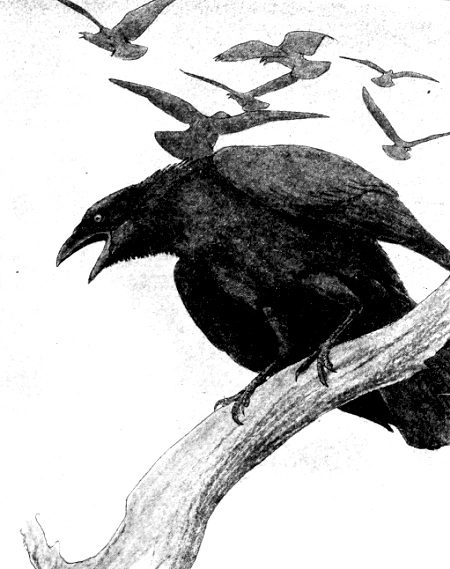
\includegraphics[scale=.5]{Crow}
  \end{center}


\NECRO[
  Name=Laughin' Jack,
  Link=necromancy-laughin-jack,
  Paradigm=Death,
  Save=N,
  Duration=0,
  Target=2
]

In a burst of blue flame and a whiff of brimstone, Laughin' Jack appears in your hand.  Jack appears as the blackened and burned skull of an infant, roughly the size of a grapefruit.  He emits a guttering, bluish corpselight from his eyes and mouth (treat as candlelight); if no one is looking at him, he whispers and chatters to himself in a language no one understands.  You may throw Jack (as a Throw weapon, obviously) using your \FOC instead of your \DEX.  Jack explodes for d4+1 damage on impact, and is able to strike creatures only hit by magic.  Throwing Jack is a Combat Action.



\NECRO[
  Name=Storm of Crows,
  Link=necromancy-storm-of-crows,
  Paradigm=Death,
  Save=Y (neg.),
  Duration=Concentration,
  Target=3
]

An inky murder of crows bursts from the ground in a whirling cloud, cloaking you and anyone Close to you.  For as long as you maintain Concentration, any ranged attacks fired into or out of the hurricane automatically miss (AoE effects like dragon's fire aren't affected).  

\mysubsection{Carnomancy}{arcana-necromancy-carnomancy}

\example{
    Using Carnomancy on an Ally requires them to make a \RS Sanity check. 
}


\NECRO[
  Name=Canopic Jar,
  Link=necromancy-canopic-jar,
  Paradigm=Death,
  Save=N,
  Duration=Session,
  Target=4
]

You pull out yours or an Ally's stomach, intestines, lungs, or liver and store them in Hammerspace.  You can only store 1 organ per person at a time.  For each person after the first, the Target increases by +1 (for example, you could store your stomach in Hammerspace, the paladin's lungs [the Target would 5], and the wizard's stomach [the Target would be 6]).  While the organ is stored in Hammerspace, you (or your Ally) are Unhallowed.  Unwilling participants get a Save.

\mybullet {
    \item \mybold{Stomach:}   You do not need to eat or drink
    \item \mybold{Intestines:}  You can heal Grit even if an effect (like a specific wound) would normally prevent you from doing so
    \item \mybold{Lungs:}  You no longer need to breathe (this makes talking impossible)
    \item \mybold{Liver:}  You are not affected by any ingested Toxins.  If performed while under the effect of the Toxin, the Toxin is removed from the body along with the liver and placed in Hammerspace.  The Toxin must be dealt with when the liver is (presumably) returned to the body.
}


\NECRO[
  Name=Corpse Tongue,
  Link=necromancy-corpse-tongue,
  Paradigm=Death,
  Save=N,
  Duration=Session or \SUMDICE Minutes,
  Target=3
]

Using Corpse Tongue requires \mylink{Corpse Salt}{necromancy-corpse-salt}

\mybullet{ 
    \item \mybold{Corpse Smoke:} The Corpse Salt is mixed with pipeweed and Smoked (eliminating its Narcotic effects).  You gain the languages, memories, and Skills of the corpse for the rest of the Session (but not any spells, supernatural abilities, Virtues, etc.).  If the creature's particularly powerful (Arbiter's discretion), you must Save vs. Hexes or gain some aspect of the creature's personality for the duration of the Session.  If the creature was over 100 years old, you must \RS : Sanity.  
    \item \mybold{Speak with Dead:}  You spread the Corpse Salt on a flat surface (be careful it doesn't blow away!)  The corpse will answer questions for \SUMDICE Minutes (the Arbiter will start a timer).  The dead only speak in Graveborn.  They will answer honestly, but the words tend to be cryptic and unhelpful, especially if the creature has no reason to help you.  Corpses usually don't remember exactly how they died.
}


\NECRO[
  Name=Covenant of Blood,
  Link=necromancy-blood-sacrament,
  Paradigm=Death,
  Save=Y (see below),
  Duration=see below,
  Target=2 (see below)
]

The Covenant of Blood allows you to do the following:

\mybullet {
    \item You can anoint someone with blood from your pricked finger.  They are Unhallowed until the end of the Session.  Unwilling creatures get a Save.
    \item Add +4 to the Target (6).  This rite can only be performed during a Bivouac.  You transfer blood from one creature to another; both creatures must be alive at the time of the transference.  Each Moment, the "donor" loses 1 point of Flesh, and the "recipient" gains 1 point of Flesh.  If the donor is brought to 0 Flesh during the transference, the recipient must Save vs Doom or fall to 0 Flesh, prompting a roll of their \DEATH
    \item Add +8 to the Target (10),  You heal from drinking another sentient creature's blood.  You may perform this liturgy during a Breather or Bivouac.  The creature must be alive when you feast on them; the act of drinking their blood takes their life.  Heal yourself to full Flesh and Grit.

}


  \begin{center}
  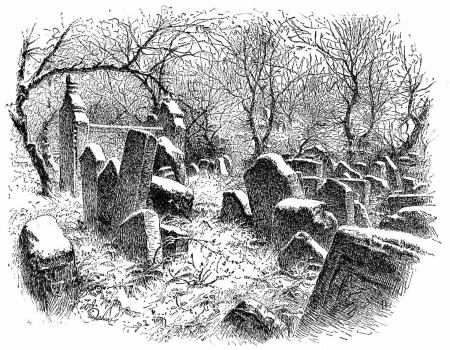
\includegraphics[scale=.5]{Graveyard}
  \end{center}


\NECRO[
  Name=Knit Flesh,
  Link=necromancy-knit-flesh,
  Paradigm=Death,
  Save=N,
  Duration=0 or Session,
  Target=2 (see below)
]

\mybullet {
    \item You heal 1 \HD of Flesh on a single creature. The healed flesh will appear gray and bloodless; wounds are sealed with wire and crude staples.  Horrible scars are usually left behind. You can only do this once per creature during a Breather or Bivouac (before you restore any Mojo).
    \item Add +1 to the Target (3).  You can remove someone's face and wear it as a mask.  You will look exactly like them (but not have their memories, skills, abilities, etc.).  The person does not need to be alive to perform this necromancy, but they do need to keep fucking still for a few minutes.
    \item Add +2 to the Target (4).  You stitch a lost limb or hand to a stump.  This requires an available limb of the appropriate size.  The limb rots quickly and a new one needs to be attached each Session.  The Mystic also can "feel" what the limb feels (i.e. they can tell if the creature is holding something [but not what], if the creature is walking or running, etc).  While the stitched limb is attached, the creature is Unhallowed.
}


\mysubsection{Corpse Witching}{arcana-necromancy-corpse-witching}

\example{
    Corpse Witching must be performed on a corpse, no more than 7 days dead (by the law of \TheAuthority).  Corpse Witching consumes (destroys) the corpse
}


\NECRO[
  Name=Corpse Salt,
  Link=necromancy-corpse-salt,
  Paradigm=Death,
  Save=N,
  Duration=0,
  Target=2
]

You create d4 \UD of Corpse Salt, a coarse and gritty distillation that can be stored in a tiny pouch or vial.  Corpse Salt is a necessary component in certain Necromantic arts, and a Narcotic sought out by Philosophers (see Narcotics under the Core Rules).


\NECRO[
  Name=Death Scythe,
  Link=necromancy-death-scythe
  Paradigm=Death,
  Save=N,
  Duration=Session or Until Exhausted,
  Target=4
]


The corpse disintegrates as you pluck a black scythe from its center of mass. The scythe is 2 Handed and does d8 damage; this d8 is a \UD - when you exhaust the \UD, the scythe disappears.  Against Monsters of the same type, the scythe has the Weapon Trait: Cleave (for example, a scythe made from a troll corpse would have Cleave against trolls.) The scythe is only usable by you and counts as a magic weapon; it does not count as a Significant Item. You must make a successful Fight check using your \FOC (instead of \VIG or \DEX) to hit with the weapon.

\NECRO[
  Name=Exploding Corpse,
  Link=necromancy-exploding-corpse,
  Paradigm=Death,
  Save=N,
  Duration=Combat,
  Target=3
]

A corpse Close or Nearby to you explodes in a shower of bone and blood.  Anyone Close to the corpse must Save vs Hexes or take \SUMDICE damage.  Makes a really big fucking mess.



\NECRO[
  Name=Zombie,
  Link=necromancy-zombie,
  Paradigm=Death,
  Save=N,
  Duration=Session or Conc.,
  Target=5
]

\mybullet{
    \item \mybold{Slave:} You raise a corpse to help with mundane tasks, test for traps, etc.  The corpse moves very slowly (d3 \MD) but doesn't need to eat, sleep, rest, or breathe.  The corpse cannot Fight or Guard, and any damage to it (including Curse the Unhallowed) immediately destroys the Zombie.  The Zombie has the strength of a normal person and can carry 25kg worth of stuff without tiring, but it'll need to be strapped to them (in a backpack or whatever).  Arbiter gets final say on what's allowed. The corpse can obey one word commands i.e. "dig", "sit", "go", "stop", etc.  The corpse can only understand Graveborn. It is completely mindless and extremely literal. The corpse will obey your last command until the spell's duration expires.  When the spell ends, the corpse falls to the ground and is immediately consumed.

    \item \mybold{Warrior:}  Creating a Warrior adds +3 to the Target (8).  The corpse is raised and will fight for you for as long as you maintain Concentration.  The Zombie uses your Mojo to Fight and Guard; you can raise as many Warriors as you wish, but they each use your Mojo to Fight and Guard. If you exhaust your Mojo or cease Concentration, the corpse falls to the ground and is immediately consumed.

}


\MONSTERBLOCK[
  Name=Zombie (Monster Stats),
  Link=necromancy-zombie-stats,
  MV=Slow*,
  WK=d20,
  DMG=2d4 1 Close,
  HD=2,
  Power=Strong,
  Soak=0,
  Morale=n/a,
  Save=2,
  Extras={Pack}
]

Zombies always go last in Combat. Zombies will try to grapple and bite automatically on following Moments. Zombie are Pack creatures (gain +1 damage for every Nearby zombie)


